\documentclass[12pt]{article}

\usepackage{sbc-template}

\usepackage{graphicx,url}

\usepackage[brazil]{babel}
%\usepackage[latin1]{inputenc}
\usepackage[utf8]{inputenc}
% UTF-8 encoding is recommended by ShareLaTex

\usepackage[algoruled,longend]{algorithm2e}
\renewcommand{\algorithmcfname}{Algoritmo}%
\renewcommand{\algorithmautorefname}{algoritmo}%
\renewcommand{\algorithmcflinename}{linha}%

\newcommand{\quotes}[1]{``#1''}

\sloppy

\title{Análise do uso de feedback de relevância no Sistema de Integração Lattes-Qualis (SILQ)}

\author{Carlos Bonetti\inst{1}
  %, Rafael H. Bordini\inst{2}, Flávio Rech
  %Wagner\inst{1}, Jomi F. Hübner\inst{3}
}

\address{Departamento de Informática e Estatística -- Universidade Federal de Santa Catarina (UFSC)\\
  Florianópolis -- SC -- Brazil
  \email{carlosbonetti.mail@gmail.com}
% \nextinstitute
%   Department of Computer Science -- University of Durham\\
%   Durham, U.K.
% \nextinstitute
%   Departamento de Sistemas e Computação\\
%   Universidade Regional de Blumenal (FURB) -- Blumenau, SC -- Brazil
%   \email{\{nedel,flavio\}@inf.ufrgs.br, R.Bordini@durham.ac.uk,
%   jomi@inf.furb.br}
}

\begin{document}

\maketitle

\begin{abstract}
   SILQ emerged in 2015 with the purpose of matching the vehicles qualified by Qualis with vehicles of publications registered on the Lattes curriculum of researchers, in order to automate the process of generating quality indicators of scientific production from these curriculums. The purpose of this work is a set of modifications to the system to include the most updated Qualis data, a study of the system's accuracy and the inclusion of controls allowing the users to suggest matchings, a technique named relevance feedback, proposing two new algorithms and an experimental analysis to evaluate their efficiency at the system.
\end{abstract}

\begin{resumo}
  O SILQ surgiu em 2015 com o objetivo de realizar o \textit{matching} automático dos veículos qualificados no Qualis com os veículos de publicações cadastradas no currículo Lattes de pesquisadores, a fim de automatizar o processo de geração de indicadores das produções contidas nesses currículos. Este trabalho propõe um conjunto de alterações no sistema para inclusão dos dados Qualis mais recentes, um estudo da taxa de acerto do sistema e a inclusão de controles que permitam ao usuário sugerir \textit{matching}, técnica denominada \textit{feedback de relevância}, propondo dois novos algoritmos e uma avaliação experimental para análise de sua eficácia no sistema.
\end{resumo}

\section{Introdução}

A Plataforma Lattes, criada e mantida pelo Conselho Nacional de Desenvolvimento Científico e Tecnológico (CNPq), é um sistema de informação responsável pela integração da base de dados de currículos, grupos de pesquisa e instituições. O Currículo Lattes se tornou o padrão nacional no registro da vida científica de estudantes, professores e pesquisadores e é hoje adotada por institutos e universidades de todo o país \cite{CNPQ-Sobre}. No Currículo Lattes pode-se inserir dados gerais do pesquisador, produção bibliográfica, orientações, citações, participações em eventos científicos entre outros dados. No módulo Produção Bibliográfica, por exemplo, é possível a inserção de artigos publicados ou aceitos para publicação em periódicos indexados pelo ISSN \cite{CNPQ-Ajuda}.

A qualidade da produção bibliográfica dos Programas de Pós-Graduação é classificada pela Coordenação de Aperfeiçoamento de Pessoal de Nível Superior (CAPES) através de um conjunto de procedimentos denominado Qualis. O Qualis define estratos de qualificação a partir da análise da qualidade dos veículos onde a produção científica de pesquisadores brasileiros foi divulgada, ou seja, periódicos e eventos científicos. Esta análise é realizada em um processo anual de atualização, sendo os veículos enquadrados nos estratos indicativos de qualidade A1, A2, B1, B2, B3, B4, B5 e C, do maior para o menor peso, para cada área do conhecimento \cite{CAPES-Classificacao}.

Apesar da Plataforma Lattes possuir um módulo de inclusão de publicações e permitir a definição do veículo onde este foi publicado, não há qualquer tipo de conexão entre os sistemas Lattes e Qualis, ou seja, o processo de avaliação de uma publicação (que é feita através da avaliação do veículo onde este foi publicado) deve ser realizado de forma manual.

O Sistema de Integração Lattes Qualis (SILQ) surgiu no ano de 2015, desenvolvido como Trabalho de Conclusão de Curso dos alunos Felipe Nedel Mendes de Aguiar e Maria Eloísa Costa do curso de Ciência da Computação da Universidade Federal de Santa Catarina (UFSC), orientados pela Prof. Carina F. Dorneles, da mesma instituição. O objetivo do sistema é a classificação automática da produção científica do currículo Lattes do pesquisador, através do \textit{matching} por similaridade de dados extraídos do Qualis, usando uma interface web amigável \cite{Silq1}.

A primeira versão do sistema foi finalizada em 2015 e desde então encontra-se disponível de forma pública e gratuita através do endereço \url{http://silq.inf.ufsc.br/}. No entanto, esta primeira versão apresenta alguns pontos que merecem melhorias.

O SILQ possui em seu banco de dados de eventos e periódicos extraídos do Qualis apenas dados referentes ao triênio 2010-2012, já que, até metade de 2015, o Qualis realizava classificações de forma trienal. Em 2016, no entanto, após a finalização do projeto SILQ, o Qualis alterou seu modo de operação para classificações anuais, já disponibilizando dados referentes aos anos 2013 e 2014, que ainda não estavam incluídos nesta primeira versão da base de dados SILQ. O primeiro ponto de melhoria é fazer com que o SILQ permita a atualização automática da qualificação a cada novo ano de lançamento do Qualis. Como o formato no qual a CAPES disponibiliza o Qualis não é interoperável, o SILQ deve oferecer esta funcionalidade.

O segundo ponto a ser trabalhado é a falta de alguns recursos que poderiam facilitar o processo de avaliação e acompanhamento de currículos, como gráficos de classificações dentro Programas de Pós-Graduação. Uma característica importante também seria a capacidade de integração com outros sistemas, facilitando o reuso do serviço disponibilizado pelo SILQ em trabalhos futuros.

O terceiro ponto de melhoria seria a avaliação experimental do algoritmo de classificação do SILQ para o estabelecimento de uma medida do grau de precisão da ferramenta. A partir disto, outras técnicas podem ser propostas e comparadas com as anteriores a fim de provar se elas resultaram em ganho de precisão.

Como o \textit{matching} entre os dados do Qualis e do Lattes de pesquisadores é feito através de funções de similaridade, o resultado pode ser um falso positivo. Portanto, um ponto importante a ser trabalhado é permitir ao usuário informar ao sistema sugestões de resultados. Esta técnica, conhecida por \textit{feedback} de relevância, exige alterar o algoritmo de classificação a fim de treiná-lo com as informações providas pelo usuário e melhorar os resultados de pesquisas similares subsequentemente realizadas. Também se faz necessária a mensuração da taxa de acerto do sistema após a inclusão desta técnica e avaliar se ela beneficia a precisão do algoritmo de classificação.

A proposta deste trabalho, portanto, é a criação de uma segunda versão do SILQ, desenvolvida a partir do código existente da primeira, a fim de realizar as mudanças sugeridas acima, junto com a atualização da base de dados e arquitetura do sistema para a inclusão das novas qualificações Qualis em um ritmo anual.

A hipótese de pesquisa a ser avaliada a partir desta ideia, portanto, é avaliar se o \textit{feedback} de usuários pode melhorar a taxa de acerto do SILQ, ou seja, aumentar o número de trabalhos corretamente avaliados pelo sistema.

\subsection{Objetivos}

O objetivo geral deste trabalho é analisar o impacto que o uso de \textit{feedback} de relevância tem na precisão dos resultados de avaliações realizadas pelo SILQ, efetuado sobre uma nova arquitetura da ferramenta que inclui a criação de API de integração com outros sistemas e a atualização da base de dados conforme as novas classificações Qualis.

Os objetivos específicos são os seguintes:

\begin{itemize}
    \item Reestruturação da arquitetura e banco de dados do SILQ a fim de suportar classificações de eventos e periódicos disponibilizados em um ritmo anual;

    \item Atualização do banco de dados do sistema com as últimas classificações disponibilizadas pelo Qualis (anos 2013 e 2014);

    \item Criação de uma API pública de disponibilização dos serviços do SILQ, via camada de aplicação REST para integração com outros sistemas;

    \item Alterações na interface do sistema incluindo migração de \textit{framework} de interface, inclusão de controles de \textit{feedback}, novos gráficos de acompanhamento de grupos de pesquisa e melhorias gerais de usabilidade;

    \item Propor novos algoritmos de avaliação baseados em similaridade textual e \textit{feedback} de relevância e verificar se a taxa de acerto do sistema foi melhorada com tal ação.
\end{itemize}

\subsection{Procedimentos Metodológicos}

A primeira etapa do trabalho envolveu a migração tecnológica da camada de interface e desacoplamento entre \textit{server} e \textit{client side}, originando um serviço \textit{RESTful} de integração. Para isto, foram utilizadas práticas ágeis de desenvolvimento de software incluindo desenvolvimento orientado a testes e eventuais modelagens lógicas de arquitetura de sistemas usando práticas da Engenharia de Software.

Concomitantemente, ocorreu a alteração da base de dados para suporte aos novos registros disponibilizados pelo Qualis. Certos aspectos do banco foram alterados para suportar tais registros novos. Os dados também passaram por um processo de \textit{data-cleaning} manual antes de serem inseridos no banco, conforme detalhado na Seção \ref{sec:extracao-qualis-novo}.

A segunda etapa do trabalho envolveu o processo de construção do módulo de captação de \textit{feedback} de relevância, envolvendo a modelagem lógica, criação da camada de serviço, API e alterações na página de resultados de avaliação do sistema com a inclusão dos controles que permitem aos usuários \quotes{julgar} os resultados retornados. Após esta etapa o algoritmo de classificação baseado em similaridade textual do SILQ foi estendido para levar em conta os \textit{feedbacks} dos usuários. Deste processo surgiram dois algoritmos que passaram por uma avaliação experimental, realizada usando um conjunto de testes contendo trabalhos extraídos de currículos Lattes de pesquisadores e manualmente avaliados por um especialista, conforme relatado na Seção \ref{sec:validation}.

\section{SILQ 2: Alterações estruturais}\label{cap:dev1}

Como já mencionado, o presente trabalho é uma continuação dos esforços iniciados por \cite{Silq1} e que deu origem ao Sistema de Integração Lattes-Qualis (SILQ). Neste capítulo será apresentado o histórico do trabalho original, os motivos e justificativas que levaram ao desenvolvimento de um novo trabalho para sua continuação, comparações do que foi alterado nesta nova versão do sistema e por que estas alterações foram necessárias.

Para mais fácil compreensão e contextualização, durante o texto serão utilizados os termos \quotes{trabalho original}, \quotes{SILQ 1} ou ainda \quotes{primeira versão do sistema} para referir-se ao trabalho de \cite{Silq1}. Os termos \quotes{SILQ 2} e \quotes{nova versão do sistema}, em contrapartida, referem-se a este trabalho.

\subsection{Histórico e Visão Geral do SILQ 1}

Este trabalho é uma continuação de \cite{Silq1}, um Trabalho de Conclusão de Curso de alunos do curso de Ciência da Computação da UFSC, orientados pela Professora Carina F. Dorneles. O objetivo desse trabalho de 2015 era a criação de um sistema que deveria ser capaz de qualificar produções científicas, nas categorias artigos e trabalhos apresentados em eventos, por busca por similaridade de dados com os dados extraídos do WebQualis \cite[p. 26-27]{Silq1}. Este objetivo foi alcançado com a criação da primeira versão do Sistema de Integração Lattes-Qualis (SILQ), lançado no segundo semestre de 2015 e disponível no sítio \url{http://silq.inf.ufsc.br/}.

Apesar de estável e com sua função principal sendo desempenhada de forma satisfatória, o SILQ 1 deixou algumas lacunas e melhorias a serem desenvolvidas por trabalhos futuros. Segundo os próprios autores, \quotes{[...] o SILQ foi concebido para ser uma ferramenta de domínio público e vários projetos devem nascer a partir dele. A continuidade do projeto só tem a acrescentar ao mundo acadêmico [...]} \cite[p. 79]{Silq1}, o que motivou a criação do trabalho para a continuação da proposta original. O ponto de partida para a nova versão do SILQ, portanto, foi a Seção \quotes{Trabalhos futuros} do trabalho original.

\subsection{Como o SILQ realiza o \textit{matching} Qualis-Lattes} \label{sec:algoritmo-silq1}

O \textit{matching} da produção científica de um currículo Lattes com o Qualis é realizado pelo SILQ com base na similaridade textual entre o título do evento de cada trabalho presente no currículo e o título do evento Qualis\footnote{O \textit{matching} por similaridade é utilizado somente para eventos. Para periódicos, o \textit{matching} é realizado através de comparação entre o ISSN informado no Lattes e nos registros Qualis.}. O título do veículo onde o trabalho foi publicado, juntamente com seu ano e área de avaliação cadastrados no Lattes são dados como \textit{query} para o sistema. O sistema busca sobre todo o conjunto de dados Qualis presentes na base de dados aquele com maior similaridade textual em relação à \textit{query}. Se esta similaridade for maior do que um \textit{threshold} pré-estabelecido, então o resultado é considerado um \textit{match} válido e o estrato atribuído pelo Qualis a este evento é também atribuído ao trabalho do pesquisador.

Pode-se tomar o exemplo real de um trabalho qualquer extraído de um currículo Lattes cujo evento tenha sido especificado como \textit{\quotes{2016 IEEE 7th Latin American Symposium on Circuits \& Systems (LASCAS)}}. A Tabela \ref{tab:exemplo-classificacao} mostra os resultados retornados pelo SILQ junto com seus respectivos valores de similaridade textual.

\begin{table}[!h]
\begin{center}
\caption{Resultados retornados pelo SILQ para a \textit{query} \textit{\quotes{2016 IEEE 7th Latin American Symposium on Circuits \& Systems (LASCAS)}}}\label{tab:exemplo-classificacao}
\begin{tabular}{ p{6cm} | c | c }
\hline
\textbf{Evento} & \textbf{Estrato} & \textbf{Similaridade} \\ \hline
IEEE Latin American Symposium on Circuits and Systems (LASCAS) & B5 & 0.87 \\ \hline
IEEE International Symposium on Circuits and Systems (ISCAS) & A1 & 0.48 \\ \hline
IEEE Latin American Robotics Symposium (LARS) & B4 & 0.45 \\ \hline
IEEE International Midwest Symposium on Circuits and Systems (MWSCAS) & B1 & 0.43 \\ \hline
Symposium on Asynchronous Circuits and Systems (ASYNC) & A2 & 0.40 \\ \hline
\end{tabular}
\end{center}
\end{table}

O primeiro resultado retornado é o escolhido, por possuir a maior similaridade em relação à \textit{query}. Neste caso, o trabalho é avaliado com o conceito B5, já que este é conceito Qualis atribuído ao evento.

O algoritmo de avaliação da primeira versão do SILQ retorna os resultados da Tabela \ref{tab:exemplo-classificacao} ao ser configurado para utilizar um \quotes{nível de confiança} de 40\%. Esse nível de confiança é o \textit{threshold} utilizado pelo algoritmo de classificação. Qualquer resultado cujo nível de similaridade em relação à \textit{query} seja inferior ao nível de confiança utilizado não é retornado.

\begin{figure}[!h]
   \centering
   \caption{Diálogo de configurações de avaliação}
   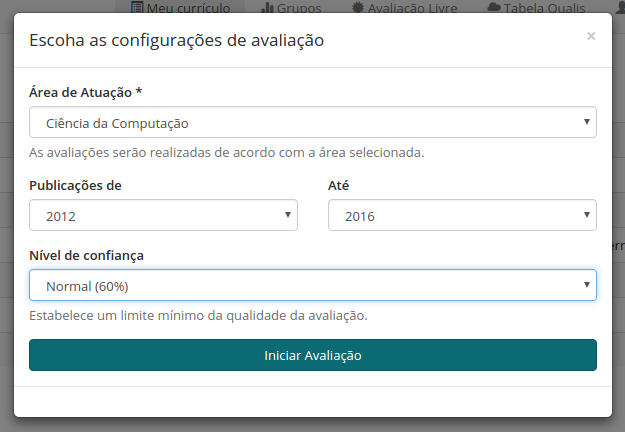
\includegraphics[width=\textwidth]{../figuras/config-avaliacao.png}
   \label{fig:config-avaliacao}
\end{figure}

O nível de confiança pode ser ajustado através das opções de avaliação, apresentadas quando o usuário requisita uma avaliação de currículo Lattes (Figura \ref{fig:config-avaliacao}). Diminuir o nível de confiança (e em consequência o \textit{threshold} do algoritmo de classificação) implica em obter mais resultados e classificar mais trabalhos, porém diminuir a precisão do algoritmo, já que resultados não relevantes serão retornados para as \textit{queries} que não obtiveram bons resultados (resultados com nível de similaridade alto). A Seção \ref{sec:validation} apresenta testes de validação do algoritmo que indicam o nível de precisão obtidos para cada valor de \textit{threshold} utilizado, além de sugerir um nível de confiança ideal a ser utilizado para maximizar o número de trabalhos corretamente avaliados pelo sistema.

\section{SILQ 2}

\subsection{Extração e inserção dos novos dados Qualis} \label{sec:extracao-qualis-novo}

Os dados Qualis de eventos e periódicos foram extraídos pelo trabalho original a partir de documentos em PDF e planilhas. Como relatado em \cite[p. 50-52]{Silq1}, os dados foram extraídos dos PDFs utilizando bibliotecas para manipulação desse formato e passaram por um processo de limpeza. A partir deste processo, aproximadamente 107 mil tuplas foram criadas representando os periódicos do triênio 2010-2012.

No primeiro semestre do ano de 2016, porém, a CAPES disponibilizou novos dados Qualis referentes ao ano de 2013 e 2014, alterando sua periodicidade de avaliação de trimestral para anual. Estes novos dados foram divulgados em formado CSV, junto com os antigos dados do triênio 2010-2012, mas desta vez separados por ano. Estes dados foram obtidos pela plataforma Sucupira (antigo WebQualis): \url{http://qualis.capes.gov.br/webqualis/}.

Como o conjunto de dados do SILQ 1 contava apenas com dados trimestrais, as tuplas originais não possuíam informação de ano (só podia-se deduzir que os dados faziam parte do triênio, mas não de qual ano). Desta forma, todas as planilhas divulgadas passaram por um novo processo de extração, incluindo os dados já inseridos no SILQ 1, mas agora considerando a nova informação de ano.

As cinco novas planilhas passaram por um processo de \textit{data cleaning} manual:

\begin{enumerate}

\item Substituição de entidades HTML especiais por seu caractere correspondente. Ex.: \quotes{\texttt{\&amp;}} por \quotes{\texttt{\&}};

\item Normalização do campo ISSN para o formato \quotes{9999-9999}: alguns registros não possuíam o dígito separador ou omitiam os zeros à esquerda;

\item Correção de ISSNs errôneos: alguns registros possuíam o campo ISSN com dígitos faltando. Ex.: 0034-167 (Revista Brasileira de Enfermagem), cujo número correto seria 0034-\textbf{7}167. Estes casos foram tratados um a um e os números corretos identificados através de pesquisas na web.

\end{enumerate}

As planilhas CSV foram então dadas como \textit{input} à base de dados resultando na criação de $339.204$ tuplas, referentes a cada um dos anos do período divulgado 2012-2015. A Tabela \ref{tab:n-registros-extraidos} mostra o número de periódicos extraídos para cada ano de avaliação do Qualis.

\begin{table}[!h]
\begin{center}
\caption{Número de periódicos extraídos dos dados Qualis}\label{tab:n-registros-extraidos}
\begin{tabular}{ c | c }
\hline
\textbf{Ano} & \textbf{Nº de periódicos extraídos} \\ \hline
2010 & 75.786 \\ \hline
2011 & 66.171 \\ \hline
2012 & 108.272 \\ \hline
2013 & 44.437 \\ \hline
2014 & 44.538 \\ \hline
\textbf{Total} & \textbf{339.204} \\ \hline
\end{tabular}
\end{center}
\end{table}

Após esta etapa, verificou-se que todos os registros da base de dados antiga do SILQ 1 estavam contidos nesta nova versão. Desta forma, os dados do SILQ 1 foram mantidos, porém agora incluindo o ano de avaliação, além do nome do periódico, ISSN, estrato Qualis atribuído pela CAPES e área de avaliação.

A inclusão dos novos registros aumentou o número de publicações passíveis de serem avaliadas pelo sistema. Os dados Qualis de 2015 e 2016 ainda não foram divulgados no momento de escrita deste trabalho, mas podem ser incluídos na base de dados, assim que forem disponibilizados pela CAPES, passando por um processo semelhante ao descrito nesta Seção.

\subsection{Criação do \textit{Web Service}} \label{sec:arquitetura-silq-2}

A primeira versão do SILQ foi desenvolvida com base no \textit{Play\footnote{\url{https://www.playframework.com/}
} Framework}, um \textit{web application framework} escrito em Java e Scala que simplifica o processo de construção de uma aplicação web. Este mesmo framework provê APIs e bibliotecas para o desenvolvimento tanto do \textit{back-end} quando do \textit{front-end} de uma aplicação web.

Para esta nova versão do SILQ, porém, um dos objetivos seria a criação de uma API de integração programática, tornando o SILQ não só um sistema para uso de usuários finais, mas também para integração com outras ferramentas, como um \textit{web service}. Para tanto, uma alteração significativa na arquitetura da aplicação foi feita, separando o sistema em um \textit{server-side} rodando Spring\footnote{\url{http://projects.spring.io/spring-framework/}} e servindo seu conteúdo através de uma API REST; e um \textit{client-side} remodelado utilizando AngularJS\footnote{\url{https://angularjs.org/}} e consumindo o serviço através de requisições HTTP.

Em um primeiro momento, o \quotes{núcleo} do SILQ, que inclui os algoritmos de avaliação e processamento dos currículos, não foi alterado, apenas a forma com que este serviço é disponibilizado e consumido. Desta forma, a linguagem utilizada no sistema, o Java, foi mantida. A escolha da alteração do framework back-end, de \textit{Play!} para \textit{Spring}, se deu ao fato da mudança no paradigma arquitetural da aplicação, com a introdução da camada REST. O Spring se trata de um framework Java \textit{open-source} largamente utilizado pela comunidade que oferece suporte a vários aspectos de uma aplicação web, incluindo a construção de interfaces RESTful.

A Figura \ref{fig:arquitetura} mostra um esquema da nova arquitetura do SILQ. A caixa \quotes{SILQ Core} representa a camada de serviço da aplicação, responsável pelo acesso ao banco de dados, avaliação de currículos e gerenciamento dos dados Qualis, cuja implementação foi realizada no trabalho passado (apesar de também sofrer algumas mudanças tecnológicas no trabalho atual).

\begin{figure}[!h]
   \centering
   \caption{Nova arquitetura do SILQ}
   \label{fig:arquitetura}
   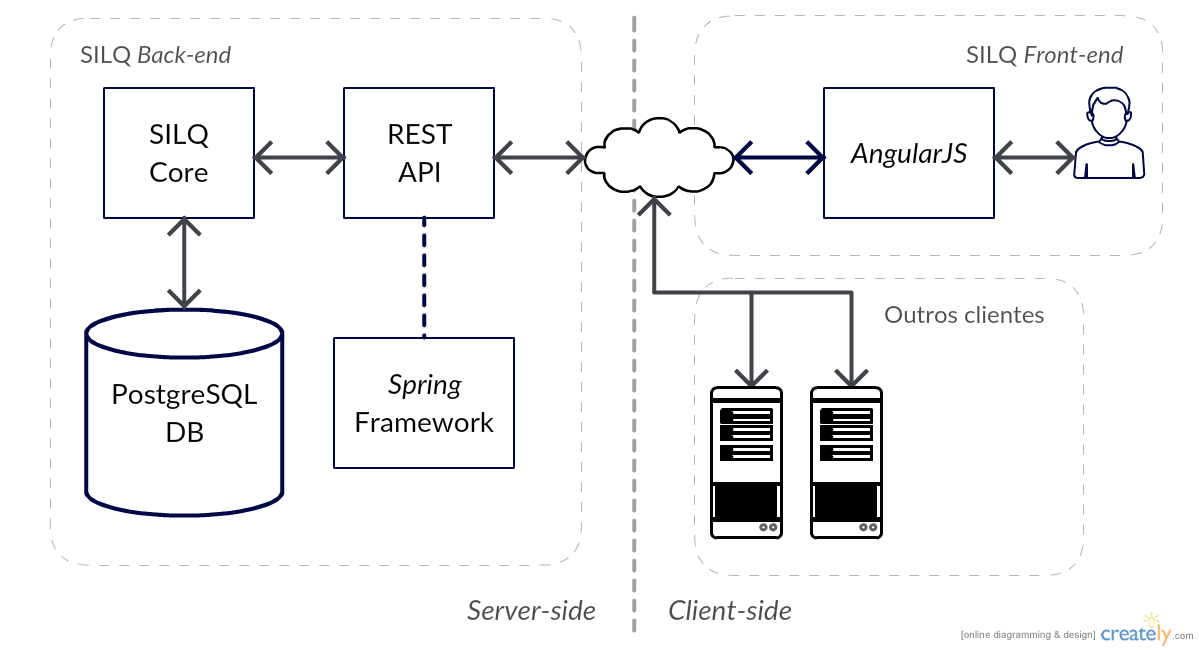
\includegraphics[width=\textwidth]{../figuras/arquitetura-silq.png}
\end{figure}

\subsection{Alterações no \textit{front-end}}

Na primeira versão do SILQ, as páginas HTML do sistema eram dinamicamente renderizadas no server-side pelo \textit{Play!} Framework e servidas conforme as requisições dos clientes. Desta forma, além de executar toda a lógica de aplicação, o servidor também fica responsável pela lógica de apresentação do conteúdo.

Em arquiteturas REST, a lógica de apresentação de dados (ou visão), fica completamente separada do servidor, executando no \textit{web browser} do cliente. O servidor só recebe requisições HTTP, as processa e retorna uma resposta em formato JSON. Esta resposta é recebida pelo cliente que então apresenta o conteúdo através da interface gráfica HTML renderizada pelo browser. Desta forma, a carga no servidor é diminuída, já que ele não está mais incumbido da tarefa de renderização das páginas HTML que serão servidas.

Utilizando esta ideia, no SILQ 2, a camada de visão foi totalmente reescrita em \textit{Javascript}, utilizando o framework \textit{AngularJS}. Trata-se de um framework \textit{open-source} desenvolvido pela Google que auxilia na criação de interfaces web dinâmicas e integração com \textit{webservices} via REST.

Desta forma, quando um cliente realiza a primeira requisição à URL do SILQ, o servidor serve uma página HTML (geralmente denominada de \textit{index}) junto com os \textit{assets} necessários para a construção de conteúdo dinâmico e estilização da página (imagens, arquivos CSS e Javascript). As requisições subsequentes, entretanto, utilizam somente requisições assíncronas ao servidor, utilizando Javascript: uma requisição conhecida por \textit{Ajax} (Asynchronous JavaScript and XML). Estas requisições utilizam a camada REST do servidor que retornará respostas em JSON e cujo conteúdo será processado no cliente e montará as páginas de forma dinâmica. Desta forma, parte da lógica da aplicação como um todo é transferida para o cliente, reduzindo a carga no servidor.

\begin{figure}[!h]
   \centering
   \caption{Página de resultados de avaliação do SILQ 1}
   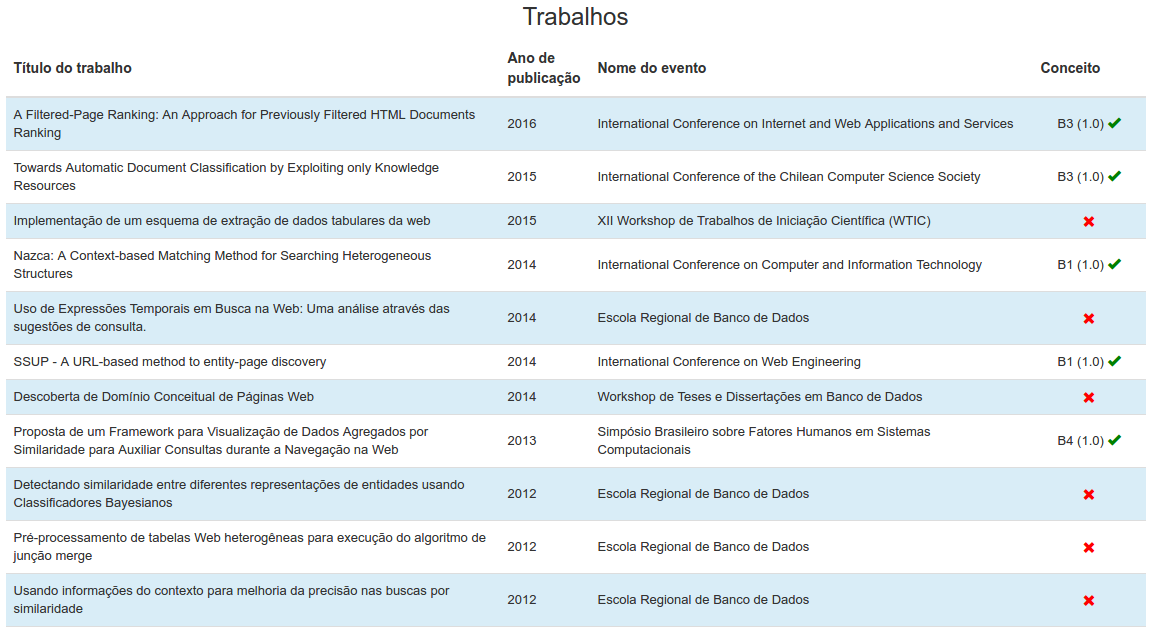
\includegraphics[width=\textwidth]{../figuras/avaliacao-silq1.png}
   \label{fig:avaliacao-silq1}
\end{figure}

\begin{figure}[!h]
   \centering
   \caption{Página de resultados de avaliação do SILQ 2}
   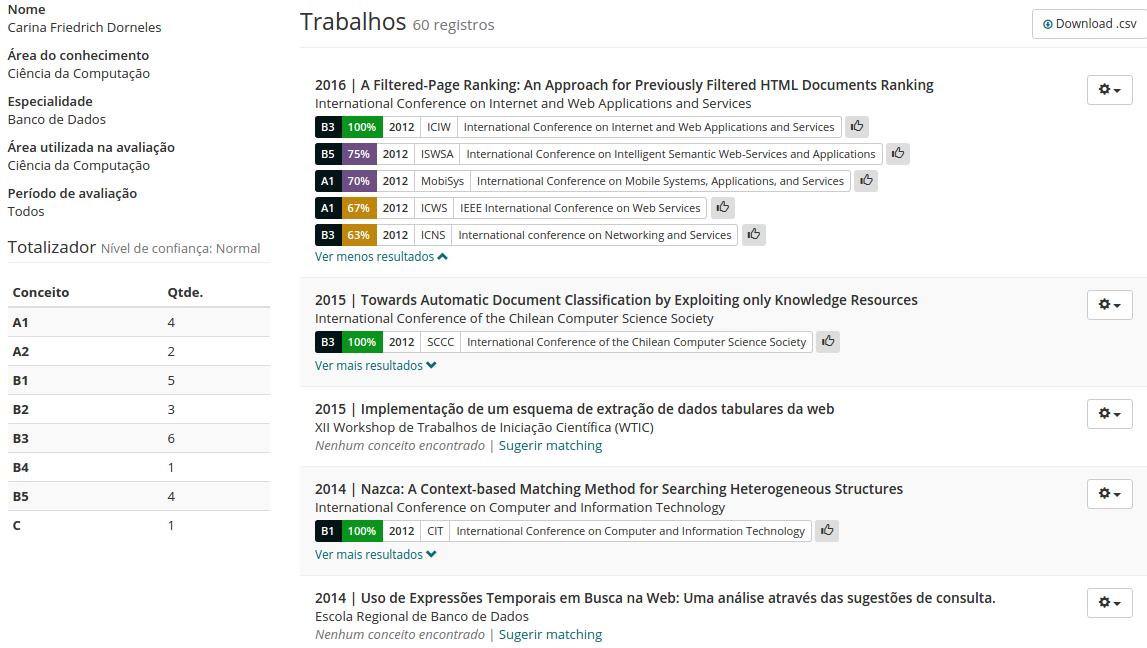
\includegraphics[width=\textwidth]{../figuras/avaliacao-silq2.png}
   \label{fig:avaliacao-silq2}
\end{figure}


Outra mudança significativa realizada no \textit{front-end} da aplicação foi a atualização do \textit{framework} CSS utilizado, inserida no processo de reescrita das páginas HTML. A primeira versão do sistema utilizava a versão 2 do \textit{framework open-source} Bootstrap\footnote{\url{http://getbootstrap.com/}}, que foi atualizada para a versão 3 no SILQ 2. De forma paralela foram realizadas algumas mudanças na interface do sistema, principalmente na página de resultados de avaliação que passou a incluir controles permitindo ao usuário informar \textit{feedback} de relevância sobre os resultados retornados. A Figura \ref{fig:avaliacao-silq1} mostra um exemplo da página de resultados de uma avaliação realizada pelo SILQ 1. A página foi remodelada para permitir a inclusão de controles de \textit{feedback} e para apresentar múltiplos resultados candidatos para um mesmo artigo ou trabalho, conforme mostra a Figura \ref{fig:avaliacao-silq2}.

\subsection{Alterações no modelo lógico}

O banco de dados relacional implementado em \textit{PostgreSQL} também sofreu algumas modificações em relação ao trabalho anterior. A Figura \ref{fig:modelo-logico} mostra o esquema lógico do banco de dados da versão atual do SILQ.

Algumas mudanças pequenas de nomenclatura foram realizadas. Uma mudança significativa, porém, foi a unificação de duas tabelas, \textit{tb\_dado\_geral} e \textit{tb\_profissional}, para uma única tabela, \textit{tb\_curriculum\_lattes}. A função destas duas tabelas antigas era guardar os currículos enviados de usuários e de pesquisadores de grupos, respectivamente. Nesta nova versão do SILQ, porém, em ambos os casos os currículos Lattes enviados pelo sistema são salvos na mesma tabela de currículos (\textit{tb\_curriculum\_lattes}), inclusive tendo seus registros reutilizados em caso de, por exemplo, dois usuários enviarem o mesmo currículo. Neste caso, o sistema armazena somente uma vez o currículo e cria duas referências diferentes a ele, poupando-o do trabalho de duplicar os dados do currículo Lattes, cuja representação em XML contém em média algumas dezenas de \textit{kilobytes}.

Outra alteração foi a adição da tabela \textit{tb\_feedback} para registro dos \textit{feedbacks} de relevância informados pelos usuários, conforme relata a Seção \ref{sec:feedback}.

\begin{figure}[!h]
   \centering
   \caption{Novo esquema do modelo lógico do SILQ}
   \label{fig:modelo-logico}
   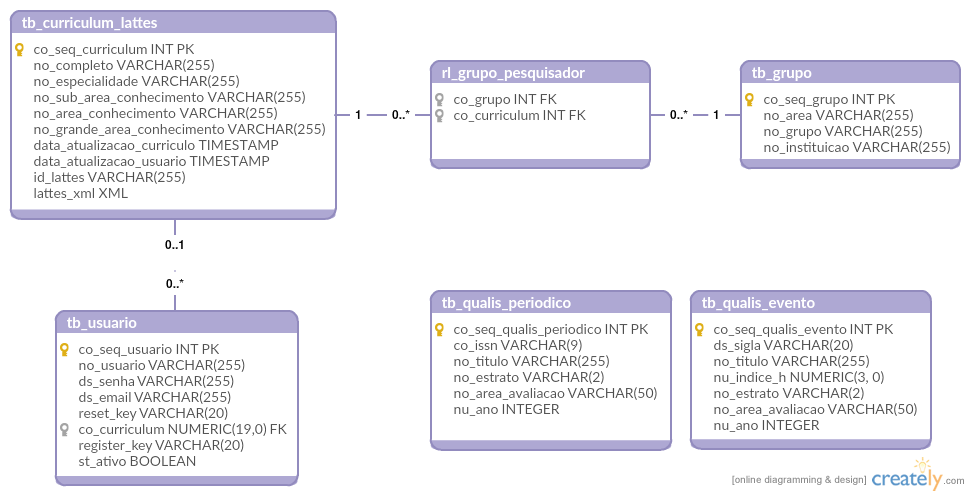
\includegraphics[width=\textwidth]{../figuras/modelo-logico.png}
\end{figure}

\subsection{Garantia da qualidade}

Para a garantia da qualidade desta nova versão do SILQ, foram introduzidas duas camadas de testes automatizados: a primeira, envolvendo \textit{testes unitários} e \textit{testes de integração} escritos em Java e com o objetivo de garantir a corretude do server-side da aplicação; e a segunda, \textit{testes de sistema} escritos em Javascript e simulando casos de uso reais, garantindo a corretude do client-side e de sua integração com o servidor.

No SILQ, os testes unitários e de integração foram escritos em Java utilizando o framework de testes \textit{jUnit}\footnote{\url{http://junit.org/}}. Eles testam cada função da camada de serviço da aplicação, por exemplo simulando o upload de um currículo qualquer e verificando se os dados extraídos e retornados são de fato aqueles contidos no currículo. Foram criados testes, inclusive, para as funcionalidades já existentes desde o SILQ 1, mas que ainda não eram cobertos com casos de teste automatizados, para assim aumentar a confiabilidade do sistema e garantir que mudanças futuras não ocasionem \textit{bugs} nestes módulos antigos.

Este nível de teste, porém, não valida a interface de usuário e sua integração com a camada de serviço. Todo o client-side da aplicação ainda estaria \quotes{descoberto} de casos de testes. Para sanar este problema, foram incluídos no SILQ casos de teste de sistema escritos em Javascript e utilizando o framework de testes \textit{Protractor}\footnote{\url{http://www.protractortest.org/}}, criado especificamente para testes \textit{end-to-end} de aplicações feitas com AngularJS. O Protractor simula as ações de um usuário real realizando cliques em botões, preenchendo formulários e navegando através de links da aplicação. Desta forma, são garantidos algum nível de corretude da interface do sistema e da integração entre o \textit{client} e \textit{server-side}.

\section{Uso de \textit{Feedback} de relevância} \label{cap:avaliacao}

Como já mencionado, um dos itens de melhoria indicados por \cite{Silq1} após a realização da primeira versão do sistema seria \quotes{permitir que o usuário auxilie a ferramenta na qualificação}. Em sistemas de IR, esta característica é denominada \textit{Feedback de Relevância}.

A ideia por trás desta técnica é permitir que o usuário julgue resultados iniciais retornados pelo sistema, classificando-os como relevantes ou não para a \textit{query} vigente. O sistema então é capaz de utilizar esta informação para melhorar seu algoritmo de classificação e retornar melhores resultados para novas \textit{queries}.

O capítulo atual apresenta como esta técnica foi aplicada no SILQ, qual modelo lógico foi utilizado para o armazenamento dos \textit{feedbacks} e qual técnica utilizada para sua obtenção. Por fim, são apresentadas medições realizadas no sistema que validam se a técnica foi relevante para o aumento da taxa de acerto do sistema.

\subsection{Obtenção de feedback} \label{sec:feedback}

Em sistemas de IR que implementam \textit{feedback} de relevância, tipicamente é permitido ao usuário julgar como relevante ou não relevante cada item retornado pelo sistema. Isso é natural pois o objetivo deste tipo de sistema é retornar a totalidade do conjunto de itens relevantes, cujo tamanho é variável dependendo da \textit{query}. O SILQ, porém, é um caso específico em que existem somente 0 ou 1 item relevante para toda \textit{query}. Isso acontece pois cada trabalho indicado no currículo Lattes de um pesquisador aparece qualificado no Qualis apenas uma única vez no ano em que o pesquisador o publicou. O objetivo do algoritmo de avaliação do SILQ é deduzir que registro Qualis é esse, caso exista na base de dados.

Para a implementação de \textit{feedback} de relevância no SILQ, portanto, não é necessário o julgamento de cada item retornado pelo sistema em uma avaliação, mas apenas marcar \textit{qual} dos itens da base de dados Qualis é um \textit{match} correto para a \textit{query} vigente. Desta forma, o usuário deve ser capaz de indicar o registro Qualis que deve ser considerado para cada trabalho avaliado. Também existe o caso especial em que não existe um registro Qualis correspondente ao trabalho, neste caso o usuário deve ser capaz de indicar que não existem \textit{matches} corretos para o trabalho.

A Figura \ref{fig:feedbacks} mostra o exemplo de três trabalhos extraídos de um currículo Lattes e avaliados pelo SILQ que receberam \textit{feedback} do usuário. O botão de \quotes{joinha} é utilizado para marcar o resultado que o usuário considera relevante para cada trabalho. Os botões grifados (com fundo azul) representam que o resultado já foi previamente marcado. Neste caso, o registro Qualis marcado como relevante é associado à \textit{query} atual, que engloba o título, ano e área do trabalho avaliado, juntamente com o usuário que está realizando o julgamento. Também é possível marcar a opção \quotes{Nenhum registro Qualis correspondente} ou sugerir algum resultado não retornado previamente pelo sistema em \quotes{Sugerir matching} (mostrado no canto inferior direito da Figura exemplo).

\begin{figure}[!h]
   \centering
   \caption{Detalhe dos controles de feedback de relevância na página de avaliação de currículo Lattes}
   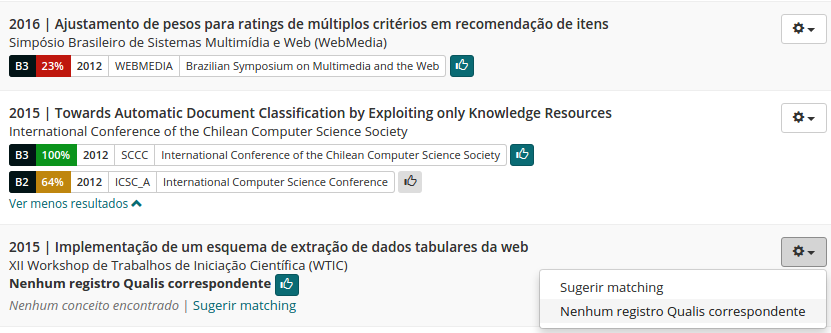
\includegraphics[width=\textwidth]{../figuras/feedbacks.png}
   \label{fig:feedbacks}
\end{figure}

Os \textit{feedbacks} de relevância dados pelos usuários são salvos na base de dados SILQ na tabela \textit{tb\_feedback} (Figura \ref{fig:modelo-logico}) para uso posterior pelo algoritmo de classificação, conforme descrito na Seção \ref{sec:algoritmo}. Já que um trabalho qualquer pode ter no máximo um registro Qualis associado, é salvo somente um \textit{feedback} por \textit{query} por usuário. Desta forma, uma chave única é utilizada na tabela de \textit{feedbacks}, dada pela dupla (título do trabalho, usuário).

\subsection{Algoritmos de avaliação com feedback} \label{sec:algoritmo}

Uma vez registrados os \textit{feedbacks} dos usuários, passa-se a questionar de que forma utilizá-los para aumentar a taxa de acerto do sistema para futuras consultas. A Seção atual apresenta dois novos algoritmos que foram propostos e avaliados neste trabalho, e como foram implementados, enquanto a próxima Seção apresenta os resultados e comparações de exatidão dos mesmos.

\subsubsection{Algoritmo \texttt{fb(t)}}

Umas das abordagens mais simples que podem ser usadas neste caso é utilizar o resultado marcado pelo usuário sempre que uma \textit{query} idêntica ao do \textit{feedback} seja submetida ao sistema. O algoritmo \texttt{fb(1.0)}, portanto, foi desenvolvido com base nesta ideia. O valor \quotes{$1.0$} presente no nome do algoritmo apenas indica que o \textit{feedback} é considerado em detrimento de qualquer outro resultado dado pelo sistema quando a \textit{query} submetida for 100\% similar (ou seja, idêntica) à \textit{query} do \textit{feedback}.

Pode-se dar o exemplo real de um nome de evento extraído de um currículo Lattes cadastrado pelo pesquisador como \quotes{Software Engineering Knowledge Engineering}, no ano de 2009 e com área de avaliação Ciência da Computação. Ao avaliar tal trabalho, o sistema retorna a lista da Tabela \ref{tab:exemplo-fb1}.

\begin{table}[!h]
\begin{center}
\caption{Resultados retornados pelo SILQ para a \textit{query} \textit{\quotes{Software Engineering Knowledge Engineering}}} \label{tab:exemplo-fb1}
\begin{tabular}{ c | p{7cm} | c }
\hline
\textbf{\#} & \textbf{Evento} & \textbf{Similaridade} \\ \hline
1 & Software Engineering and Data Engineering (SEDE) & 0.53 \\ \hline
2 & International Conference on Software Engineering and Knowledge Engineering (SEKE) & 0.49 \\ \hline
3 & Software Engineering and Applications (SEA\_A) & 0.45 \\ \hline
... & ... & ... \\
\hline
\end{tabular}
\end{center}
\end{table}

Após analisar esta lista, o usuário submeteu um \textit{feedback} ao sistema marcando o resultado \#2 como o correto. Desta forma, utilizando o algoritmo \texttt{fb(1.0)}, toda \textit{query} subsequente idêntica a \quotes{Software Engineering Knowledge Engineering} terá o resultado \#2 retornado na primeira posição.

O \texttt{fb(1.0)} considera apenas \textit{feedbacks} que sejam idênticos à \textit{query} submetida, \textit{queries} similares não são consideradas. O usuário do exemplo anterior possui um outro trabalho cadastrado em seu currículo Lattes cujo título de evento é \quotes{Software Engineering \textbf{and} Knowledge Engineering}. Pode-se deduzir que o usuário quis se referir ao mesmo evento, porém o título não é idêntico ao exemplo anterior por causa do termo \textit{\quotes{and}}. Neste caso, o algoritmo \texttt{fb(1.0)} não é capaz de deduzir que os dois casos se referem ao mesmo evento, apesar da semelhança entre eles. Uma modificação que pode ser realizada no algoritmo é utilizar uma função de similaridade entre novas \textit{queries} submetidas ao sistema com aquelas anteriormente submetidas e que possuem \textit{feedback} do usuário. Se a similaridade entre a nova \textit{query} e algum dos \textit{feedbacks} for maior do que certo \textit{threshold de feedback}, então é provável que a nova \textit{query} se refira ao mesmo evento do \textit{feedback} anteriormente fornecido.

O algoritmo \texttt{fb(t)} (para $0.0 \le t \le 1.0$) é uma generalização de \texttt{fb(1.0)} que considera \textit{feedbacks} cuja similaridade textual em relação à \textit{query} seja maior que o \textit{treshold} $t$. Por exemplo, \textit{fb(0.75)} irá considerar \textit{feedbacks} cujo valor de similaridade textual em relação à \textit{query} seja $0.75$ ou superior. No exemplo anterior, ao submeter a nova \textit{query} \quotes{Software Engineering and Knowledge Engineering} ao sistema, o algoritmo \textit{fb(0.75)} calcula a similaridade entre ela e os \textit{feedbacks} anteriores fornecidos pelo usuário e encontra o \textit{feedback} da primeira \textit{query} \quotes{Software Engineering Knowledge Engineering} por ser 88\% similar à \textit{query} atual. Neste caso, por ter uma similaridade maior do que o \textit{threshold} de $0.75$ estipulado, o algoritmo retorna o mesmo evento marcado no \textit{feedback} para a \textit{query} atual (o evento \#2 da Tabela \ref{tab:exemplo-fb1}).

O algoritmo \texttt{fb(t)}, entretanto, leva a outros questionamentos, já que utiliza a mesma técnica de \textit{data-matching} que foi proposta a melhorar. Qual o valor de $t$ (\textit{treshold de feedback}) ideal? Qual o algoritmo de similaridade textual ideal para este caso? A Seção \ref{sec:avaliacao-algoritmos} apresenta testes de validação do algoritmo \texttt{fb(t)} para diferentes valores de $t$.

O Algoritmo \ref{alg:fbt} é a representação em pseudocódigo de \texttt{fb(t)}. O parâmetro $q$ representa a \textit{query}, $t$ é o valor de \textit{threshold de feedback}, $D$ é o conjunto de todos os documentos a serem pesquisados e $F$ o conjunto de \textit{feedbacks} fornecidos contendo as duplas ($q_f, d$), \textit{query} do \textit{feedback} e documento dado como \textit{feedback}, respectivamente, tal que $d \in D$. A variável $m$ é o registro provindo de \textit{feedback} com maior probabilidade de ser um \textit{match} correto para a \textit{query}, caso exista. A saída $R$ é uma lista 0-indexada contendo os resultados da consulta, ordenada por ordem decrescente da probabilidade do resultado ser um \textit{match} correto para a \textit{query}. A função \texttt{trigram\_sim} calcula a similaridade textual entre duas \textit{strings} utilizando o método \textit{trigrams} e retornando um valor no intervalo $[0, 1]$. A função \texttt{trigram\_rank} é o algoritmo de avaliação da primeira versão do SILQ, que cria o rank $R$ de similaridade a partir da comparação entre $q$ e cada um dos documentos de $D$. A função \texttt{insert\_rank\_top} insere um registro no topo do \textit{rank}, removendo itens duplicados previamente inseridos.

\begin{algorithm}
\caption{\texttt{fb(t)}}
\label{alg:fbt}
\LinesNumbered
\SetKwInOut{Input}{Input}\SetKwInOut{Output}{Output}
\SetAlgoLined
\Input{$q, t, D, F$}
\Output{$R$}

$R \gets \texttt{trigram\_rank(q, D)}$

$s_m \gets -1$

\For{$ (q_f, d) \in F$}{
   $s \gets \texttt{trigram\_sim($q, q_f$)}$

	\If{$s \ge t$ \texttt{and} $s \ge s_m$}{
		$m \gets d$

    $s_m \gets s$
	}
}

\If{$m$}{
  $\texttt{insert\_rank\_top(R, m)}$
}

\KwRet{$R$}
\end{algorithm}

\subsubsection{Algoritmo \texttt{query\_aliasing}}

Uma adaptação de \texttt{fb(t)} que mostrou-se de mais fácil implementação e que não gera o questionamento de qual valor de $t$ utilizar, foi considerar as \textit{queries} de \textit{feedbacks} anteriormente fornecidos pelo usuário, da mesma forma que o \texttt{fb(t)}, porém inseri-las no \textit{rank} de resultados de novas \textit{queries} submetidas com base em seus valores de similaridade textual em relação à nova \textit{query}, junto com os resultados previamente selecionados. Assim, ao invés de escolhê-lo em detrimento dos demais, o evento marcado com \textit{feedback} só é retornado se for mais bem ranqueado que os demais resultados.

Considerando os mesmos exemplos dados na Seção anterior, em que o usuário submete a nova \textit{query}  \quotes{Software Engineering and Knowledge Engineering} ao sistema, o algoritmo de \texttt{query\_aliasing} realiza comparação textual entre a nova \textit{query} e as \textit{queries} anteriores que possuam \textit{feedback}, da mesma forma que o \texttt{fb(t)}, encontrando a \textit{query} \quotes{Software Engineering Knowledge Engineering}, com um valor de similaridade de $0.88$. Ao contrário do $fb(t)$, o algoritmo de \texttt{query\_aliasing} irá inserir o evento dado como \textit{feedback} a esta \textit{query} junto com a lista de resultados previamente encontrados apenas via similaridade textual, usando o valor de $0.88$ para posicionamento no \textit{ranking}. A Tabela \ref{tab:exemplo-qa} mostra o \textit{ranking} retornado para este exemplo. Nota-se que o evento \#2, marcado pelo usuário como correto, foi elevado no \textit{ranking} por receber o novo valor de similaridade da comparação com o \textit{feedback}.

\begin{table}[!h]
\begin{center}
\caption{Resultados retornados pelo SILQ para a \textit{query} \textit{\quotes{Software Engineering and Knowledge Engineering}} utilizando \texttt{query\_aliasing}} \label{tab:exemplo-qa}
\begin{tabular}{ c | p{7cm} | c }
\hline
\textbf{\#} & \textbf{Evento} & \textbf{Similaridade} \\ \hline
2 & International Conference on Software Engineering and Knowledge Engineering (SEKE) & 0.88 \\ \hline
1 & Software Engineering and Data Engineering (SEDE) & 0.62 \\ \hline
3 & Software Engineering and Applications (SEA\_A) & 0.53 \\ \hline
... & ... & ... \\ \hline
\end{tabular}
\end{center}
\end{table}

O valor de similaridade atribuído, porém, perde seu significado semântico pois não é mais a similaridade textual entre o título do evento do Lattes e do Qualis calculado através do \textit{trigrams}, mas um valor adimensional usado apenas para ordenação relativa dentro do \textit{ranking}.

Desta forma, ao processar uma \textit{query} $q$ qualquer, o sistema processa um \textit{rank} de resultados primários com base no algoritmo \textit{trigrams} inicial. O \textit{rank} é ordenado do resultado mais similar à $q$ ao menos similar. Após esta etapa, ele também compara $q$ com cada uma das \textit{queries} anteriormente submetidas pelo usuário e que possuem \textit{feedback} de relevância utilizando o mesmo algoritmo de similaridade textual. O resultado mais similar é inserido no \textit{ranking} de resultados. Assim, se $q$ é idêntico a um \textit{feedback} já submetido pelo usuário, o evento deste \textit{feedback} será retornado e inserido no topo do \textit{ranking} de resultados, por ser 100\% similar à \textit{query}. Outros resultados similares, porém não idênticos, serão inseridos no \textit{ranking} conforme seu valor de similaridade e só serão escolhidos em detrimento de outros resultados primários se seus valores de similaridade forem superiores a eles.

É como se, ao dar um \textit{feedback} de relevância qualquer, o usuário criasse um \textit{alias} (um apelido) ao resultado que está sugerindo. Assim, o sistema deve avaliar novas \textit{queries} não só comparando-as com o nome real dos documentos, mas também com os apelidos dados a eles pelo usuário. Por este motivo o algoritmo foi chamado de \texttt{query\_aliasing}. A avaliação deste algoritmo foi realizada e comparada com os demais na Seção \ref{sec:avaliacao-algoritmos}.

O Algoritmo \ref{alg:qa} é a representação em pseudocódigo do método proposto. O significado semântico das variáveis é equivalente ao do Algoritmo \ref{alg:fbt}. A saída deste algoritmo é o próprio \textit{rank} $R$, possivelmente contendo novos resultados devido à comparação com os \textit{feedbacks} de $F$. O método \texttt{insert\_rank} da linha \ref{lin:insert} insere o registro $d$ na lista ordenada $R$ com um valor de \textit{rank} $s$, preservando a ordenação da lista, de forma que o elemento em $R[0]$ seja aquele com maior valor de \textit{rank} e, assim, o registro com maior probabilidade de ser um \textit{match} correto para a \textit{query}. A função também elimina itens duplicados, preservando aquele com maior valor de \textit{rank}.

\begin{algorithm}
\caption{\texttt{query\_aliasing}}
\label{alg:qa}
\LinesNumbered
\SetKwInOut{Input}{Input}\SetKwInOut{Output}{Output}
\SetAlgoLined
\Input{$q, D, F$}
\Output{$R$}

$R \gets \texttt{trigram\_rank(q, D)}$

\For{$ (q_f, d) \in F$}{
   $s \gets \texttt{trigram\_sim($q, q_f$)}$

   $\texttt{insert\_rank(R, s, d)}$ \label{lin:insert}
}
\KwRet{$R$} \label{li:sum-zero-begin}
\end{algorithm}

\subsection{Avaliação experimental} \label{sec:validation}

Esta Seção apresenta os procedimentos realizados para avaliar as alterações promovidas no algoritmo de avaliação da nova versão do SILQ e se elas contribuíram para o aumento da taxa de acerto do sistema.

\subsubsection{Conjunto de testes}

O conjunto de testes utilizado para a avaliação do sistema foi criado a partir dos currículos Lattes de 33 pesquisadores do programa de pós-graduação em Ciência da Computação da Universidade Federal de Santa Catarina (UFSC).

Destes 33 currículos, 300 publicações foram selecionadas de forma aleatória e manualmente avaliadas: caso possuíssem um registro Qualis equivalente então a publicação juntamente com o Qualis associado eram salvos no conjunto de testes; caso não possuíssem registro Qualis equivalente, então eram marcados como tal e também adicionados ao conjunto de testes.

Nas avaliações descritas a seguir, foram dadas como \textit{query} ao sistema cada uma das publicações da coleção de testes, porém sem expor os resultados manualmente avaliados. Cada resposta retornada pelo sistema foi comparada com a respectiva resposta manualmente selecionada. Em caso das respostas serem idênticas, então o sistema avaliou corretamente a publicação; em caso de não serem idênticas, avaliou incorretamente. O caso de não haver registro Qualis equivalente à publicação foi considerada uma resposta correta quando o sistema não retornou nenhum resultado, e uma resposta incorreta caso contrário.

\subsubsection{Métricas utilizadas}

Uma vez definido o conjunto de teste, é preciso definir as métricas utilizadas na avaliação. Através da comparação das métricas é possível concluir se houve melhora em certos aspectos do sistema. No caso do SILQ, deseja-se melhorar a taxa de acerto, ou seja, maximizar o número de trabalhos corretamente avaliados. As métricas clássicas de avaliação de sistemas IR discutidas na Seção \ref{sec:avaliacao-ir} foram consideradas.

As métricas de precisão e revocação foram descartadas por não se encaixarem com a forma de avaliação do sistema, baseada em \textit{rank}. Conforme já discutido, estas métricas não são indicadas para sistemas deste tipo. Medidas mais indicadas nesse caso são \textit{Precision at k} (\textit{P@k}) e \textit{R-Precision}. O algoritmo de avaliação do SILQ, porém, considera apenas o primeiro registro Qualis retornado para realizar \textit{match} com o trabalho sendo avaliado (apenas o mais similar). Neste caso, a avaliação usando estas duas métricas devem considerar apenas o primeiro resultado, ou seja, \textit{P@1} e \textit{R-Precision} com $|R| = 1$ (sendo $R$ o número de registros relevantes para a \textit{query}). Em ambos os casos, para cada \textit{match} retornado pelo sistema, temos medidas com valor igual a 0, caso o sistema não tenha avaliado corretamente o trabalho, e 1 caso tenha avaliado corretamente. Têm-se, portanto, um simples valor \textit{booleano} indicando se houve acerto ou não, para cada \textit{query} submetida. Considerando todo o conjunto de testes, pode-se somar o número de acertos e dividir pelo tamanho do conjunto, resultado um valor que indica a \textit{taxa de acerto} do sistema. Este valor também é conhecido como \textit{exatidão}\footnote{O termo utilizado na literatura é \textit{accuracy}, cuja tradução usual é \textit{precisão}. Optou-se pelo uso do termo \textit{exatidão}, no entanto, para evitar confusões com a métrica de precisão.} e foi a medida base escolhida para a  avaliação experimental do sistema.

Outra medida utilizada em um primeiro momento foi a Média de Rank Recíproco (MRR). Conforme discutido, ela é particularmente interessante para sistemas que produzem uma lista de resultados ordenados por probabilidade de corretude, e, ao contrário da exatidão, é capaz de modelar o quão bem o sistema classificou o resultado correto, mesmo quando ele não foi classificado em primeiro lugar.

Por estas razões, as medidas de exatidão (ou taxa de acerto) e MRR foram escolhidas para as avaliações experimentais descritas nas próximas subseções.

\subsubsection{Avaliação de \textit{threshold} ideal}

 Um dos questionamentos levantados no início deste trabalho e que geralmente ocorre ao projetar sistemas de \textit{data matching} baseados em similaridade, é o de qual \textit{threshold} utilizar. Na primeira versão do sistema foi introduzido um controle de \quotes{nível de confiança} que permitia ao usuário controlar o \textit{threshold} utilizado pelo algoritmo, conforme detalhado na Seção \ref{sec:algoritmo-silq1}. O nível de confiança padrão, porém, foi fixado em 60\% (equivalente ao \textit{threshold} de valor $0.6$). Este valor foi provavelmente escolhido de forma empírica pois observou-se que maximizava o número de resultados corretos, porém não foram realizados experimentos comprovando esta teoria.

 Desta forma, para encontrar o valor de \textit{threshold} ideal foi utilizado o conjunto de testes para avaliar o algoritmo inicial do SILQ 1, em um primeiro momento. O método utilizado foi o de avaliar via sistema cada uma das publicações do conjunto de testes e comparar com o resultado real, e repetir o processo variando o \textit{threshold} a fim de observar as médias de exatidão e de rank recíproco (MRR). Os resultados foram agrupados no gráfico da Figura \ref{fig:avaliacao-threshold}. A linha em azul claro representa a exatidão, ou seja, a taxa de trabalhos corretamente avaliados pelo sistema. A linha em cinza representa a média de rank recíproco (MRR), calculada conforme discutido na Seção \ref{sec:mrr}.

 \begin{figure}[!h]
    \centering
    \caption{Taxa de trabalhos corretamente avaliados e Média de Rank Recíproco (MRR) para diferentes \textit{thresholds}}
    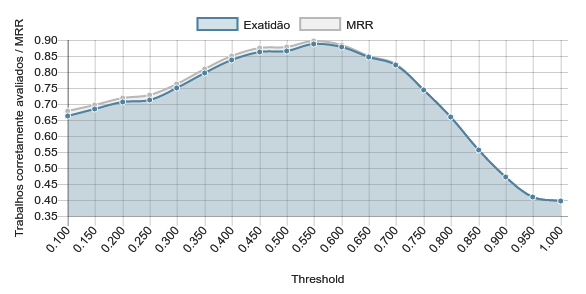
\includegraphics[width=\textwidth]{../figuras/avaliacao-threshold.png}
    \label{fig:avaliacao-threshold}
 \end{figure}

O primeiro fenômeno que observamos ao avaliar o gráfico é o ponto de máximo por volta do valor $0.55$ de \textit{threshold}, que totaliza uma exatidão aproximada de 88\%, e a tendência da exatidão baixar ao se afastar deste pico, para ambas as direções. Esse é um comportamento esperado pois valores de \textit{threshold} baixos tendem a diminuir a exatidão do sistema por retornar resultados não relevantes para as \textit{queries}, enquanto valores altos tendem a diminuir a exatidão por deixar de retornar resultados relevantes. Este ponto máximo trata-se, portanto, do \textit{threshold} ideal para o caso de testes em questão.

Outra característica observada é a tendência do valor de MRR acompanhar o da exatidão, sendo sempre igual ou apenas um pouco superior em magnitude. Isso acontece pela forma com que o MRR é calculado, atribuindo valor de $1/r$ a cada avaliação, sendo $r$ a posição em que o resultado real foi avaliado pelo sistema. Se o resultado foi corretamente avaliado, portanto, o valor de $1/1 = 1$ é atribuído ao resultado, o mesmo valor que seria atribuído à exatidão, já que o conjunto de valores possíveis para esta métrica é $\{0, 1\}$ para cada resultado (0 representando um erro e 1 representando um acerto). A semelhança dos valores, portanto, indica que houveram poucos casos em que o algoritmo retornou o resultado real em posições inferiores à primeira no \textit{rank} de avaliação. Esta característica do valor de MRR permaneceu constante nos demais testes realizados neste trabalho, portanto omitiu-se o valor de MRR nas demais avaliações.

\subsubsection{Avaliação dos algoritmos} \label{sec:avaliacao-algoritmos}

Os algoritmos descritos na Seção \ref{sec:algoritmo} foram avaliados utilizando o mesmo processo descrito na Seção anterior. O algoritmo \textit{trigrams} trata-se do método inicial utilizado pelo SILQ 1 e cuja análise de \textit{threshold} ideal foi realizada na Seção anterior. O algoritmo \texttt{fb(t)} foi testado variando $t$ nos valores que obtiveram melhores resultados. Todas as análise foram realizadas com valor de \textit{treshold} igual a $0.55$. A Tabela \ref{tab:comparacao-algoritmos} apresenta os resultados de cada teste.

\begin{table}[!h]
\begin{center}
\caption{Comparação da exatidão dos diferentes algoritmos testados (utilizando \textit{threshold} de $0.55$)}
\label{tab:comparacao-algoritmos}
\begin{tabular}{ c | c }
\hline
\textbf{Algoritmo} & \textbf{Exatidão} \\
\hline

\textit{trigrams} & 88.667\% \\
\textit{fb(1.00)} & 89.667\% \\
\textit{fb(0.90)} & 90.667\% \\
\textit{fb(0.80)} & 92.667\% \\
\textit{fb(0.70)} & 92.667\% \\
\textit{fb(0.60)} & 91.000\% \\
\textit{query\_aliasing} & \textbf{93.333}\% \\

\end{tabular}
\end{center}
\end{table}

A primeira tentativa de usar \textit{feedback} de relevância na avaliação foi com o algoritmo \textit{fb(1.00)}, que considera os resultados informados pelo usuário quando a \textit{query} é idêntica a algum \textit{feedback}. Houve uma melhora na taxa de acertos, porém de forma não tão significativa.

As variações que utilizam valores menores de $t$, porém, obtiveram melhores resultados, por serem capazes de identificar \textit{queries} similares aos \textit{feedbacks} já informados pelo usuário, mesmo quando este não julgou exatamente a \textit{query} em questão. Um exemplo que demonstra este fato são os nomes de eventos \textit{\quotes{IEEE International Symposium on Computer-Based Medical Systems}} e \textit{\quotes{27th International Symposium on ComputerBased Medical Systems (CBMS)}}, extraídos de um mesmo currículo Lattes. É fácil notar que tratam-se do mesmo evento, porém o usuário informou a sigla e o número da edição no segundo, e nenhuma destas informações no primeiro (além de não utilizar o hífen em um dos casos). Caso o usuário tenha dado \textit{feedback} para somente um dos casos, os algoritmos \texttt{fb(t)} com valores de $t$ inferiores a $1.0$ são capazes de utilizar o mesmo \textit{feedback} para ambos, apesar das \textit{queries} não serem idênticas.

Valores de $t$ muito baixos, porém, deterioram rapidamente a taxa de acerto pois consideram \textit{feedbacks} similares entre eventos que não tem relação. Desta forma, existe também um \quotes{valor ideal} de $t$, que gira em torno de $0.7$ a $0.8$ conforme os testes realizados.

O algoritmo \texttt{fb(t)}, porém, pode cometer \quotes{injustiças} pois considera os \textit{feedbacks} como resultados corretos, independente dos resultados primários retornados, caso sejam superiores ao \textit{threshold} $t$. O algoritmo de \texttt{query\_aliasing} resolve este problema inserindo o \textit{feedback} no \textit{ranking} junto com os demais resultados. O melhor resultado (aquele mais similar à \textit{query}) será utilizado, independente da técnica usada para obtê-lo. Nos testes realizados, o algoritmo de \texttt{query\_aliasing} obteve a melhor taxa de acerto, com uma média de 93.3\% de trabalhos corretamente avaliados.

Foi realizada uma última avaliação comparativa entre o algoritmo \textit{trgm} inicial e o novo que utiliza \texttt{query\_aliasing}. A Figura \ref{fig:avaliacao-algoritmos} mostra a taxa de acerto média para ambos os algoritmos variando o \textit{threshold} utilizado. Nota-se que o algoritmo que utiliza \textit{feedback} de relevância obteve melhores resultados, para qualquer \textit{threshold} utilizado, aumentando em aproximadamente 6\% a taxa de acerto. O \textit{threshold} ideal, porém, se manteve constante em $0.55$ pois é dependente da função de similaridade.

\begin{figure}[!h]
   \centering
   \caption{Comparação da taxa de acerto do algoritmo \textit{trgm} e do \textit{trgm + query\_aliasing} para diferentes \textit{thresholds}}
   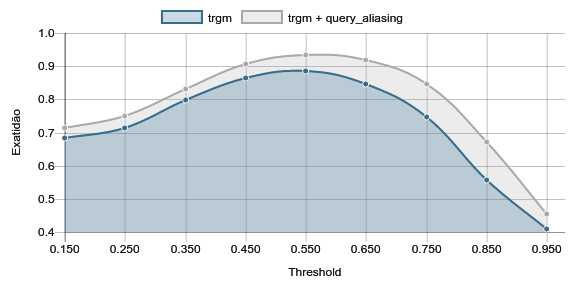
\includegraphics[width=\textwidth]{../figuras/avaliacao-algoritmos.png}
   \label{fig:avaliacao-algoritmos}
\end{figure}

\section{Conclusões e trabalhos futuros}

O SILQ é um esforço coletivo para a automatização e consequente melhoria na qualidade de gestão de grupos de pesquisa e principalmente de Programas de Pós-Graduação. A atualização tecnológica e alimentação da base de dados da ferramenta são processos que devem ser constantemente realizados para mantê-la viável aos seus usuários.

Os objetivos iniciais de refatoração arquitetural com inclusão de melhorias de interface, novas funcionalidades e criação da camada de integração REST, foram alcançados. Tanto usuários como desenvolvedores de aplicações interessados no sistema se beneficiam dessa alteração. Também foram realizadas as inclusões de controles permitindo sugestões de resultados por parte dos usuários, e desenvolvidos dois algoritmos que utilizam tais informações para melhorar a taxa de acerto do sistema.

A hipótese de pesquisa levantada se mostrou verdadeira. De fato foi possível aumentar a precisão do sistema utilizando \textit{feedback} de relevância dos usuários. Isso se mostrou verdade por meio dos experimentos realizados e relatados neste trabalho, e com o teste dos algoritmos propostos.

A avaliação de \textit{threshold} mostrou que o valor ideal para o SILQ é de aproximadamente $0.55$, muito próximo do \quotes{nível de confiança normal} estabelecido no trabalho anterior de \cite{Silq1}, e que a taxa de acerto para este caso é de 88\%.

Os algoritmos \texttt{fb(t)} e \texttt{query\_aliasing}, baseados em \textit{feedback} de relevância e similaridade textual, foram propostos e avaliados experimentalmente. Ambos resultaram em melhoria na taxa de acerto do sistema. O algoritmo \texttt{query\_aliasing} foi preferido por resultar em uma melhor precisão e ser de mais fácil implementação, e está atualmente em uso na versão 2.3 do sistema. Através da alteração do \textit{threshold} ideal e da inclusão do algoritmo baseado em \textit{feedback} de relevância, a taxa de acerto média do sistema aumentou de 87\% para 93.3\%.

Esses resultados são relevantes não só por mostrarem que a taxa de acerto média do sistema aumentou, mas por estabelecerem uma medida base para trabalhos futuros. Os algoritmos utilizados neste trabalho são estratégias simples de uso de \textit{feedback} de relevância construídas sobre a mesma função de similaridade textual do SILQ 1, o método \textit{trigrams}, porém outros algoritmos e estratégias diferentes podem ser testados. Em especial, ambos algoritmos propostos consideram apenas o conjunto de \textit{feedbacks} de um usuário específico, de forma a evitar a necessidade do tratamento de \textit{feedbacks} conflitantes ou divergentes de diferentes usuários.

Como trabalhos futuros pode-se sugerir os seguintes itens:

\begin{itemize}

\item Propor e analisar outros métodos de similaridade textual ou estratégias diferentes que possam melhorar ainda mais a precisão do SILQ. Alguns exemplos seriam o uso de \textit{machine learning} para treino do algoritmo de classificação, uma estratégia conhecida por \textit{learning to rank}; e o algoritmo de \textit{Rocchio}, muito utilizada em sistemas que implementam \textit{feedback} de relevância e baseado no modelo de espaço vetorial;

\item Considerar \textit{feedbacks} provindos de terceiros, ou seja, levar em conta \textit{feedbacks} informados por outros usuários, mesmo que o atual não tenha informado \textit{feedback} a respeito de uma \textit{query} específica;

\item Considerar nomes de eventos traduzidos. Comumente são utilizados nomes de periódicos ou eventos estrangeiros em inglês no currículo Lattes, porém em português no Qualis, ou vice-versa. Esses casos dificilmente são avaliados corretamente pelo sistema, já que o algoritmo atual é baseado em comparação por similaridade textual;

\item Levantamento da produção por veículo de publicação. Considerando todos os currículos cadastrados no SILQ, seria possível levantar o número de publicações em cada periódico e evento cadastrado no Qualis;

\item Gerar os valores de $I_{restrito}$ e $I_{geral}$ automaticamente. Tratam-se de índices definidos pela CAPES e utilizados na avaliação de Programas de Pós-Graduação;

\item Considerar, para fins de ponderação dos valores de estrato Qualis, os pesos considerados pela avaliação de Programas de Pós-Graduação realizada pela CAPES.

\end{itemize}

As mudanças relatadas neste trabalho já se encontram disponíveis na página oficial do SILQ: \url{http://silq.inf.ufsc.br/}, na versão 2.3 no momento de escrita deste trabalho, porém em constante evolução.

\section{References}

\bibliographystyle{sbc}
\bibliography{artigo}

\end{document}
